\Chapter{Hasonló alkalmazások és koncepció}

\Section{Mesterséges intelligencia a videojátékokban}
A mesterséges intelligencia már több mint fél évszázada foglalkoztatja az embereket, mind a tudományos fantasztikus regényekben, mind az informatikában, ambár az utóbbi az viszonylag újkeletű dolog. Az első definíció, és maga a fogalom mint mesterséges intelligencia (artificial intelligence) egy amerikai informatikustól John McCarthytól származik, 1956ból{\cite{ai}}.
%ref: https://courses.cs.washington.edu/courses/csep590/06au/projects/history-ai.pdf

Videojátékok terén is az 50es évekre tehető a kezdet, 1950ben mutatták be a "Bertie the Brain" nevezetű számítógépet, mely segítségével mesterséges intelligencia ellen lehetett játszani a Tic-tac-toe nevezetű játékot. Egy évre rá 1951ben kiadták a Brit Nimrod nevezetű számítógépet ahol szintén gépi ellenfél ellen lehetett megmérkőzni, de ezúttal a Nim nevű játékban.
Ezek a számítógépek elég kezdetlegesek voltak nem is biztos hogy mára már hagyományos értelemben véve videojátéknak neveznénk őket, de kétségkívül az elsők között voltak, akik MI-t használtak ilyen célra.
%ref: https://en.wikipedia.org/wiki/Bertie_the_Brain
%ref: https://en.wikipedia.org/wiki/Nimrod_(computer)

Az első kísérletek után nem kellett sokat várni hogy az eddiginél komolyabb szoftvereket tudjanak írni, erősebb gépi ellenfelekkel, amelyek az évtized végére, és a 60as évek elejére még tovább fejlődtek. Ugyanakkor a 70es évekig kellett várni olyan nagy címekre, mint a \textit{Spacewar!} és a \textit{Pong}, majd az évtized végén megjelenő \textit{ Space Invaders (1978)} és \textit{Pacman (1980)}, melyeknél már fokozatosan erősödtek a gépi ellenfelek.
A 80as és 90es években már szinte minden zsánerben fellelhető volt valamiféle mesterséges intelligencia, legyen szó verekedős, stratégiai, sport, vagy szerepjátékról.

Természetesen sokakban kritika is megfogalmazódott, hogy nem-e úgy vannak leprogramozva a gépi ellenfelek hogy csaljanak, és gyakran ez igaz is volt, mert egyszerűbb egy stratégiai játékban olykor olykor megadni az MI-nek a valódi játékos pozicíóját, mint leprogramozni ténylegesen hogy megtalálja. Gyakori szokás még szintén stratégiai játékokban hogy valamennyi százalék bónuszt kap egy-egy nyersanyagra az ellenfél. Habár a kritika teljesen jogos, és néhol tényleg látványos ez a csalás, manapság sokkal kifinomultabbab ezek a rendszerek, és a lehető legjobb játélélményt szolgálják, mivel szinte elengedhetetlenné vált a videojáték iparban a mesterséges intelligencia használata.

Felmerül ugyanakkor a kérdés, hogy amennyiben egy videojátékba be lehet programozni egy mesterséges intelligenciát ami ellenfélnek (vagy csapattársnak) szolgál az emberi játékos számára, meg lehet-e tanítani vagy be lehet-e programozni egy másik MI-t arra hogy játszon egy játékkal? A továbbiakban ezzel a kérdskörrel fogunk foglalkozni.

\Section{A Warcraft játékmechanikája}

2 faj közül lehet választani, ember és ork. Mivel egy korai játékról van szó, a fajok között csak kozmetikai különbségek vannak, mindegy egységnek és épületnek megvan a másik fajba tartozó párja, és még a statisztikái is ugyan azok. Ez egy olcsó mód arra hogy egyensúlyban legyen a két faj így nem befolyásolja különösebben a játék lefolyását.

Játékmódokat tekintve létezik kampány mód, melyben fajonként 12 küldetésben ismerhetjük meg a Warcraft történetét. Ebben segítenek minket az átvezető videók, és az egyedi kialakítású pályák, hogy a lehető legjobban bele tudja magát élni az ember.
Egy másik, szabadabb játékmód az egyedi játék, ahol mi magunk választhatjk hogy milyen pályán akarunk játszani, milyen fajjal és az ellenfelünk ki legyen. Ez utóbbit megtehetjük többjátékos módban is.

Bármelyik módot is választjuk, célunk ugyan az, le kell győznünk az ellenséget, de hogy is érhetjük ezt el? Természetesen katonákat kell képeznünk akik parancsunkra elvégzik a feladatot, amihez infrastruktúra kell, ahhoz pedig nyersanyag. Utóbbiból 2 féle létezik, a fa és az arany, melyet az adott fajunknak megfelelő munkások szerezhetnek. Fákat az erdők kivágásával szerezhetünk, aranyat pedig az aranybányákból, amit gyakran nekünk kell megtalálni, ezzel nehezítve a folyamatot. 

Figyelni kell ugyanakkor arra is, hogy legyen elég lakhely az embereinknek, amit farmok építésével lehet növelni. Az építési mechanizmus nem bonyolult, habár korlátozott, ugyanis csak épület és út közelében lehet építeni, így előbb az utat kell kiépíteni, ami aranyba kerül, és csak ez után lehetséges az épületek felhúzása. Különböző épületek más-más szerepet töltenek be és más egységeket lehet képezni bennük. 

A felfedezésnek is nagy szerepe van az ilyen stílusú játékban, ugyanis kezdetkor csak a térkép minimális részére van rálátásunk, így érdemes néhány egységgel felfedezni. Ebben a játékban ez különösen fontos, ugyanis a játék kora miatt még nem létezett az úgynevezett "Fog of War", aminek a lényege, hogy nem látható a pálya minden része, csak az, ami a játékos által irányított egységek/épületek látómezejében van. Így a Warcraftban hatalmas előny a felfedezett terület, mert így folyamatosan lehet figyelni az ellenséges mozdulatokat.

\begin{figure}[h]
    \centering
    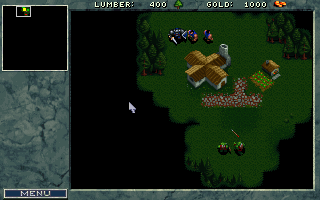
\includegraphics[scale=1]{images/wc.png}
    \caption{A fázisok lépései}
    \label{fig:warcraft}
\end{figure}

\Section{Ember a gép ellen}
\subsection{AlphaStar}
Talán a legjobb eredményt a Deepmind mesterséges intelligenciája érte el a StarCraft II nevű játékban, mely jelenleg jobb a játékosok 99,8\%-nál{\cite{deepmind}}. 
%ref:https://www.theverge.com/2019/10/30/20939147/deepmind-google-alphastar-starcraft-2-research-grandmaster-level
Ez a játék talán a legkomplexebb a jelenlegi stratégiai játékok közül, nem hiába fektetnek komoly pénzeket a verseny szintű mérkőzések lebonyolítására.
Léteztek már az AlphaStar előtt is MI-k amik képesek voltak valamilyen szinten játszani, de azok valamiféle előnyt kaptak a cél elérése érdekében, például egyszerűsített pályák, korlátozott játékmenet, emberfeletti képességek, így azok teljesítménye közel sem éri el az elvárt szintet.

Nagy probléma továbbá leküzdeni azt, hogy egyszerűbb játékokkal szemben (mint például a Tic-tac-toe vagy a kő-papír-olló) nincsen úgymond "legjobb stratégia", így rengeteg esetet kell vizsgálni és folyamatosan új módszereket keresni. Ugyanígy a már említett táblás játékokhoz való hozzáállást sem lehet alkalmazni, mert amíg a sakkban és a goban minden információ adott, egy ilyen stratégiai játékban rengeteg a rejtett, ismeretlen tényező, amelyet fel kell fedezni. Mindezt nehezíti hogy ezt valós időben, vagy legalábbis minimális késlekedéssel kell elemezni és döntést hozni, ráadásul figyelembe venni a hosszú távú tervezést is. Ugyanígy a sakkal ellentétben, ahol csak 6 féle bábú van, és egyszerre maximum 32 játszik egy adott mérkőzésen, egy videojátékban több tucat egység variáns lehet, amelyekből több száz is létezhet egyidejűleg, ezzel növelve a komplexitást.

\subsection{A StarCraft és a Warcraft}
Mivel mind a két játékot a Blizzard készítette, rengeteg hasonlóság fedezhető fel bennük, ha mind a kettőből az eredeti, első részt vesszük, rájövünk hogy igazából a Starcraft az csak egy továbfejlesztett Warcraft másolat, sci-fi köntösbe bújtatva, és a fajok közötti különbséget már nem csak kinézetben kereshetjük, hanem az egységek statisztikái, és a különböző fajok játékstílusa is más. Ezt a legjobban egy táblázattal lehetne szemléltetni.

A győzelem úgy érhető el, hogy megsemmisítjük az összes ellenséges egységet és épületet.
\begin{table}[h]
    \centering
    \caption{Összehasonlítás}
    \label{tab:osszehasonlitas}
    \begin{tabular}{|c|c|c|}
    \hline
    ~ & Warcraft & Starcraft \\
    \hline
    Megjelenés & 1994 & 1998 \\
    Játszható fajok száma & 2 & 3 \\
    Fajonként eltrérő egység statisztika & nem & igen \\
    Játszható pályák száma & 20 & 86 \\
    \hline
    \end{tabular}
\end{table}

Látható hogy már a régebbi StarCraft is hatványozottabban komplexebb volt az spirituális elődjénél, így érthető hogy az utódhoz évekbe telt olyan intelligenciát írni, ami szinte mindekit legyőz.


\Section{A Terv}

Mindazok után hogy megnéztük az MI kialakulását a videojátékok terén, továbbá a hasonló alkalmazások jellemzőit, eredményeit. Ideje tervet készíteni, milyen lépések szükségesek ahhoz hogy implementálni lehessen egy Warcraft-al játszó mesterséges intelligenciát.

Általánosságban elmondható, hogy az elkészítendő intelligenciát pythonban szeretnénk megvalósítani, részeredményeket és statisztikákat karakteres felületen közöljük a felhasználóval, és zavartalanul kell futnia magának a játéknak is.

\subsection{1. lépés: DosBox forráskódjának megismerése}

Mielőtt hozzáfognánk magához a mesterséges intelligenciához, a Warcraftot futtató emulátor forráskódjával kell megismerkedni. Fel kell tennünk magunknak néhány kérdést, amelyet majd az implementáció során igyekszünk megválaszolni, így megoldva a problémákat.

\begin{itemize}
    \item Hogyan tudjuk irányítani a billentyűzetet és az egeret?
    
    Eléggé evidens ennek a kérdésnek a létjogosultsága, valamilyen úton-módon hozzá kell férnünk a kurzor pozíciójához és a billentyűzethez és mindezt magában a kódban irányítani.  
    \item Melyik kódrész az ahová beilleszthetjük a saját kódrészünket?
    
    Ezt talán az egyik legnehezebb megtalálni, mivel elég terjedelmes programról van szó, és csak úgy akárhova nem előnyös beilleszteni kódot, mert nem tudhatjuk milyen hatást fejtünk ki az emulátorra. A meghatározáshoz gondos előkészületek kellenek, és a lehető legkevesbé kell lassítani a programot.
\end{itemize}

\subsection{2. lépés: Képernyőkép mentése}

\begin{itemize}
    \item Hogyan mentsük le a képet? Esetleg van rá beépített függvény?
    
    Itt elsődlegesen beépített függvény(eknek) kell utána nézni, amennyiben nincsen, vagy nem használható, eldönteni hogy fájlba írást kellene megvalósítani, vagy egészen más megoldást keresni.
    \item Milyen időközönként kellene ezt megtenni?
    
    Optimális időintervallumot kell találni a Képernyőkép rögzítésére, ami nem túl rövid ahhoz hogy lehetetlenség legyen az összeset feldolgozni, és rá választ kapni, ugyanakkor nem is túl hosszú, hogy darabosnak tűnjön tőle a játékmenet, és feleslegesen várakozzon bemenetre az MI.
\end{itemize}

\subsection{3. lépés: Processzek közötti kommunikáció}

\begin{itemize}
    \item Hogyan fog a lementett kép bekerülni az MI-be?
    
    Ez a kérdés erősen függ az előző ponttól. Amennyiben a fájlba mentés megoldható, és a mentési intervallul is elfogadható, akkor csak be kell olvasnia az MI-nek a lementett fájlt. Ugyanakkor ha ez nem megoldható, más módszerek után kell nézni.  
    
    \item Hogyan fogunk választ küldeni a DosBoxnak hogy hova kell kattintani?
    
    Amennyiben feldolgoztuk a képet, és megvan hova kell kattintani/mit kell megnyomni, kérdéses hogy ezt hogyan juttatjuk vissza a DosBoxba. Ez is működhete-e fájlba írással, vagy ennél elegánsabb módszert kell találni.  

\end{itemize}


\subsection{4. lépés: Adatfeldolgozás}

\begin{itemize}
    \item Hogyan ismeri fel a mesterséges intelligencia hogy mit is lát pontosan?
    
    Ez is megoldható többféleképpen, amennyiben rendelkezésre állnak a játékban használt spriteok, abban az esetben az úgynevezett template matching is alkalmazható. Amennyiben ez nem járható út, akkor valamiféle becslés alapján kell meghatározni az éppen látni vélt objektumot.
    % ref: https://en.wikipedia.org/wiki/Template_matching

    \item Mi alapján dönt a következő lépésről?
    
    Ennek a lépésnek ez a legnehezebb része. Történhet a döntéshozatal úgy, hogy kvázi előre bele van programozva egy stratégia, és azt próbálja végrehajtani, vagy öntanuló algoritmus alapján is. Az utóbbi elegánsabb, ugyanakkor kérdéses hogy elbír-e ez a módszer egy ilyen komplexitású játékot, annak ellenére hogy mai szemmel nem tekinthetjük annak. 
\end{itemize}



